% Gerado automaticamente. No preambulo do documento use:
% \usepackage{pgfplots}
% \pgfplotsset{compat=1.18}
\definecolor{plotblue}{HTML}{2563EB}
\definecolor{plotorange}{HTML}{D97706}
\definecolor{plotgreen}{HTML}{059669}
\definecolor{plotpurple}{HTML}{7C3AED}
\definecolor{plotgray}{HTML}{374151}
\definecolor{plotred}{HTML}{DC2626}
\definecolor{plotteal}{HTML}{0F766E}
\definecolor{plotslate}{HTML}{64748B}

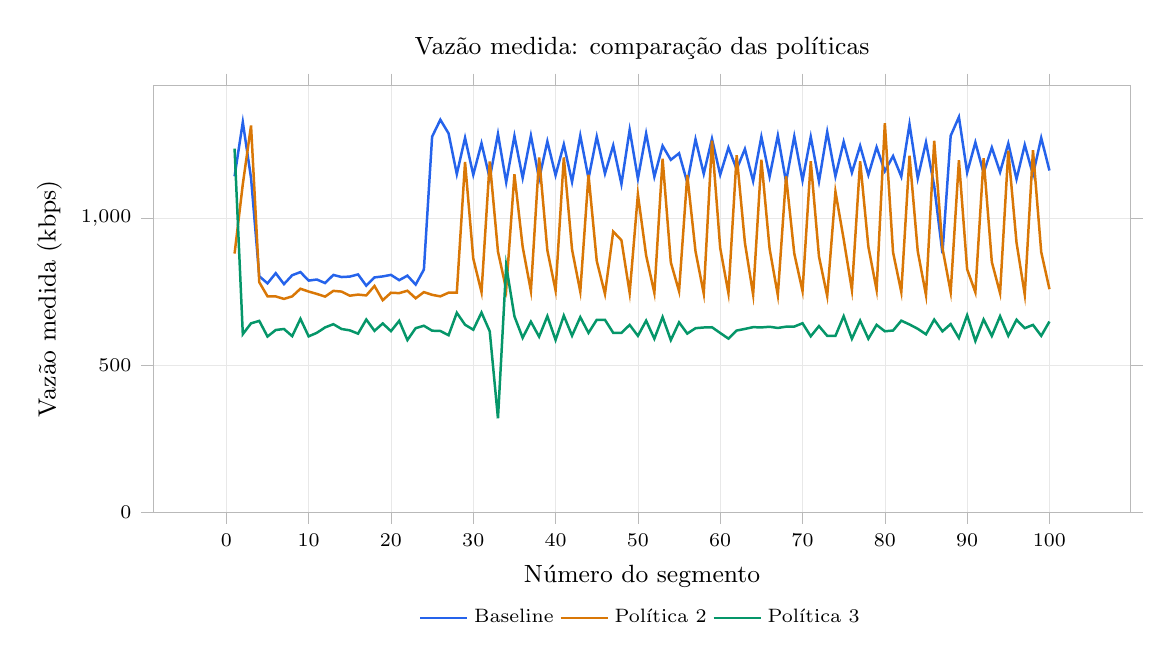
\begin{tikzpicture}
\begin{axis}[
    title={Vazão medida: comparação das políticas},
    xlabel={Número do segmento},
    ylabel={Vazão medida (kbps)},
    width=14cm,
    height=7cm,
    grid=major,
    grid style={line width=.12pt, draw=gray!18},
    axis line style={draw=gray!55},
    tick style={draw=gray!55},
    tick align=outside,
    title style={font=\small},
    label style={font=\small},
    tick label style={font=\scriptsize},
    legend cell align={left},
    legend style={at={(0.5,-0.20)}, anchor=north, legend columns=3, draw=none, font=\scriptsize},
    ymin=0,
    ymax=1453.73
]
\addplot+[plotblue, line width=0.9pt, mark=none] coordinates {
(1,1143.95)
(2,1328.54)
(3,1138.18)
(4,803.55)
(5,779.31)
(6,813.9)
(7,776.71)
(8,806.99)
(9,817.64)
(10,788.74)
(11,792.33)
(12,780.3)
(13,808.01)
(14,800.8)
(15,802.36)
(16,809.8)
(17,771.28)
(18,799.55)
(19,802.93)
(20,808.17)
(21,790.17)
(22,805.51)
(23,775.11)
(24,826.37)
(25,1279.19)
(26,1336.91)
(27,1290.04)
(28,1151.62)
(29,1275.14)
(30,1149.32)
(31,1256.44)
(32,1136.78)
(33,1288.3)
(34,1123.63)
(35,1281.4)
(36,1138.63)
(37,1282.65)
(38,1134.98)
(39,1263.17)
(40,1147.59)
(41,1252.75)
(42,1125.01)
(43,1282.76)
(44,1136.76)
(45,1279.06)
(46,1153.33)
(47,1249.03)
(48,1117.68)
(49,1302.46)
(50,1136.21)
(51,1289.81)
(52,1142.6)
(53,1247.8)
(54,1200.18)
(55,1222.35)
(56,1122.79)
(57,1270.05)
(58,1152.65)
(59,1272.04)
(60,1149.34)
(61,1241.64)
(62,1168.11)
(63,1237.03)
(64,1127.87)
(65,1278.56)
(66,1143.15)
(67,1282.93)
(68,1125.11)
(69,1279.8)
(70,1130.02)
(71,1278.61)
(72,1127.05)
(73,1295.46)
(74,1143.96)
(75,1261.52)
(76,1156.48)
(77,1247.96)
(78,1148.67)
(79,1243.1)
(80,1161.66)
(81,1212.87)
(82,1143.09)
(83,1321.32)
(84,1137.56)
(85,1259.92)
(86,1111.08)
(87,881.67)
(88,1282.07)
(89,1346.05)
(90,1156.73)
(91,1259.5)
(92,1155.33)
(93,1241.68)
(94,1158.25)
(95,1256.09)
(96,1134.58)
(97,1251.19)
(98,1149.3)
(99,1275)
(100,1163.95)
};
\addlegendentry{Baseline}
\addplot+[plotorange, line width=0.9pt, mark=none] coordinates {
(1,880.71)
(2,1117.29)
(3,1317)
(4,783.19)
(5,735.22)
(6,734.76)
(7,726.35)
(8,734.94)
(9,761)
(10,751.33)
(11,743.3)
(12,734.17)
(13,753.68)
(14,751.23)
(15,737.19)
(16,741.02)
(17,738.21)
(18,770.34)
(19,721.84)
(20,747.31)
(21,745.99)
(22,754.15)
(23,728.45)
(24,749.44)
(25,740.15)
(26,734.95)
(27,747.43)
(28,747.8)
(29,1192.69)
(30,863.63)
(31,749.34)
(32,1194.82)
(33,887.55)
(34,758.78)
(35,1150.81)
(36,903.75)
(37,753.62)
(38,1208.59)
(39,891.9)
(40,755.07)
(41,1208.62)
(42,894.43)
(43,751.06)
(44,1149.04)
(45,855.79)
(46,743.22)
(47,955.83)
(48,926.17)
(49,746.73)
(50,1082.37)
(51,874.4)
(52,746.79)
(53,1203.77)
(54,850.8)
(55,752.35)
(56,1148.25)
(57,888.44)
(58,744.46)
(59,1265.26)
(60,899.51)
(61,745.32)
(62,1215.72)
(63,917.82)
(64,740.9)
(65,1200.35)
(66,897.24)
(67,738.79)
(68,1144.52)
(69,880.54)
(70,753.17)
(71,1195.25)
(72,870.69)
(73,736.11)
(74,1091.62)
(75,929.95)
(76,756.48)
(77,1195.46)
(78,904.22)
(79,757.09)
(80,1325.23)
(81,885.12)
(82,749.69)
(83,1213.82)
(84,888.57)
(85,739.46)
(86,1264.92)
(87,899.68)
(88,749.4)
(89,1198.72)
(90,827.33)
(91,748.82)
(92,1205.41)
(93,851.93)
(94,745.98)
(95,1231.27)
(96,918.13)
(97,740.93)
(98,1232.75)
(99,885.96)
(100,759.54)
};
\addlegendentry{Política 2}
\addplot+[plotgreen, line width=0.9pt, mark=none] coordinates {
(1,1238.31)
(2,606.31)
(3,643.05)
(4,651.44)
(5,598.12)
(6,620.36)
(7,623.82)
(8,599.42)
(9,658.41)
(10,598.63)
(11,610.83)
(12,629.25)
(13,640.16)
(14,623.74)
(15,619.19)
(16,607.86)
(17,656.04)
(18,617.51)
(19,642.64)
(20,616.5)
(21,651.64)
(22,586.17)
(23,626.61)
(24,634.86)
(25,618.02)
(26,616.95)
(27,602.48)
(28,679)
(29,638.26)
(30,621.3)
(31,679.84)
(32,615.83)
(33,319.21)
(34,839.59)
(35,666.84)
(36,593.84)
(37,648.65)
(38,597.57)
(39,667.44)
(40,586.38)
(41,669.19)
(42,600.97)
(43,664.1)
(44,610.58)
(45,655.14)
(46,655.03)
(47,610.73)
(48,610.69)
(49,637.76)
(50,600.4)
(51,652.08)
(52,590.59)
(53,664.39)
(54,585.86)
(55,646.36)
(56,608.04)
(57,626.6)
(58,628.88)
(59,629.79)
(60,610.21)
(61,590.99)
(62,618.53)
(63,624.04)
(64,630.09)
(65,629.16)
(66,631.34)
(67,627.29)
(68,631.69)
(69,632.1)
(70,643.37)
(71,598.95)
(72,633.7)
(73,600.47)
(74,600.42)
(75,667.26)
(76,590.48)
(77,652.31)
(78,590.63)
(79,637.81)
(80,616.02)
(81,618.56)
(82,652.15)
(83,639.21)
(84,624.43)
(85,605.63)
(86,655.77)
(87,615.78)
(88,640.56)
(89,593.15)
(90,670.43)
(91,583.01)
(92,656.16)
(93,600.23)
(94,667.34)
(95,600.52)
(96,655.21)
(97,626.66)
(98,637.74)
(99,600.48)
(100,649.2)
};
\addlegendentry{Política 3}
\end{axis}
\end{tikzpicture}
